%==============================================================================
%  Design Thinking & Fabrication Laboratory
%  A detailed LaTeX Beamer presentation covering the full 5-unit syllabus.
%
%  Build:  pdflatex main.tex   (run twice for the table of contents / navigation)
%  Figures are generated by  scripts/generate_figures.py  into  figures/
%==============================================================================
\documentclass[aspectratio=169,11pt]{beamer}

\usepackage[T1]{fontenc}
\usepackage[utf8]{inputenc}
\usepackage{lmodern}
\usepackage{textcomp}
\usepackage{amssymb}
\usepackage{graphicx}
\usepackage{tikz}
\usepackage{booktabs}
\usepackage{newunicodechar}
\usetikzlibrary{shapes.geometric,arrows.meta,positioning,calc}

% ---- map a few Unicode glyphs so raw characters compile under pdflatex --------
\newunicodechar{→}{$\rightarrow$}
\newunicodechar{←}{$\leftarrow$}
\newunicodechar{↔}{$\leftrightarrow$}
\newunicodechar{×}{$\times$}
\newunicodechar{·}{\textperiodcentered}
\newunicodechar{–}{--}
\newunicodechar{—}{---}
\newunicodechar{★}{$\star$}
\newunicodechar{✓}{\checkmark}

%==============================================================================
%  COLOUR PALETTE  (matches the generated figures)
%==============================================================================
\definecolor{dtink}{HTML}{22333B}
\definecolor{dtnavy}{HTML}{264653}
\definecolor{dtteal}{HTML}{2A9D8F}
\definecolor{dtblue}{HTML}{2A6F97}
\definecolor{dtsky}{HTML}{61A5C2}
\definecolor{dtyellow}{HTML}{E9C46A}
\definecolor{dtorange}{HTML}{F4A261}
\definecolor{dtcoral}{HTML}{E76F51}
\definecolor{dtplum}{HTML}{7B506F}
\definecolor{dtmoss}{HTML}{6A994E}
\definecolor{dtpaper}{HTML}{FBF9F5}
\definecolor{dtcloud}{HTML}{EDF2F4}
\definecolor{dtgrey}{HTML}{5B6B73}

%==============================================================================
%  CUSTOM (theme-less) LOOK
%==============================================================================
\useinnertheme{rectangles}
\setbeamercolor{normal text}{fg=dtink,bg=white}
\setbeamercolor{structure}{fg=dtblue}
\setbeamercolor{frametitle}{fg=white,bg=dtnavy}
\setbeamercolor{title}{fg=dtnavy}
\setbeamercolor{item}{fg=dtteal}
\setbeamercolor{subitem}{fg=dtorange}
\setbeamercolor{subsubitem}{fg=dtblue}
\setbeamercolor{block title}{fg=white,bg=dtblue}
\setbeamercolor{block body}{fg=dtink,bg=dtcloud}
\setbeamercolor{alerted text}{fg=dtcoral}
\setbeamercolor{section in toc}{fg=dtnavy}
\setbeamercolor{palette primary}{fg=white,bg=dtnavy}

\setbeamerfont{frametitle}{series=\bfseries,size=\large}
\setbeamerfont{title}{series=\bfseries,size=\Huge}
\setbeamerfont{block title}{series=\bfseries}
\setbeamerfont{section in toc}{series=\bfseries}

% bullets
\setbeamertemplate{itemize item}{\raisebox{0.15ex}{\small$\blacktriangleright$}}
\setbeamertemplate{itemize subitem}{\textcolor{dtorange}{\textbullet}}
\setbeamertemplate{itemize subsubitem}{\textcolor{dtblue}{\textopenbullet}}
\setbeamertemplate{navigation symbols}{}

% ---- frame title as a coloured band -----------------------------------------
\setbeamertemplate{frametitle}{%
  \nointerlineskip
  \begin{beamercolorbox}[wd=\paperwidth,ht=3.2ex,dp=1.4ex,leftskip=0.6cm,rightskip=0.6cm]{frametitle}%
    \usebeamerfont{frametitle}\insertframetitle%
    \hfill\raisebox{-0.3ex}{\textcolor{dtyellow}{\small\insertframenumber}}%
  \end{beamercolorbox}%
  \vspace*{0.15cm}%
}

% ---- coloured accent rule below content title -------------------------------
\newcommand{\accentrule}{\textcolor{dtorange}{\rule{\linewidth}{1.2pt}}}

% ---- simple footline --------------------------------------------------------
\setbeamertemplate{footline}{%
  \leavevmode\hbox{%
  \begin{beamercolorbox}[wd=.5\paperwidth,ht=2.2ex,dp=1ex,leftskip=.3cm]{palette primary}%
    \tiny Design Thinking \& Fabrication Laboratory%
  \end{beamercolorbox}%
  \begin{beamercolorbox}[wd=.5\paperwidth,ht=2.2ex,dp=1ex,rightskip=.3cm]{palette primary}%
    \hfill\tiny\insertsectionhead%
  \end{beamercolorbox}}%
}

%==============================================================================
%  HELPER MACROS
%==============================================================================
% coloured keyword
\newcommand{\kw}[1]{\textbf{\textcolor{dtblue}{#1}}}
\newcommand{\kwc}[1]{\textbf{\textcolor{dtcoral}{#1}}}
\newcommand{\kwt}[1]{\textbf{\textcolor{dtteal}{#1}}}

% a figure that fills most of a frame, with an optional caption line
\newcommand{\bigfig}[2]{%
  \begin{center}
    \includegraphics[height=0.74\textheight,width=\linewidth,keepaspectratio]{figures/#1}\\[0.2em]
    {\small\itshape\textcolor{dtgrey}{#2}}
  \end{center}}

% coloured "pill" label
\newcommand{\pill}[2]{\tikz[baseline=(x.base)]{\node[fill=#1,text=white,rounded corners=3pt,inner sep=2.5pt,font=\bfseries\footnotesize](x){#2};}}

% section divider frame
\newcommand{\unitdivider}[3]{% number, title, subtitle
  \begingroup
  \setbeamercolor{background canvas}{bg=dtnavy}
  \begin{frame}[plain]
    \centering
    \vfill
    {\tikz\node[fill=dtorange,text=white,circle,minimum size=1.7cm,font=\bfseries\Large]{#1};}\\[0.5em]
    {\usebeamerfont{title}\color{white}\bfseries #2}\\[0.4em]
    {\color{dtyellow}\large #3}\\[0.3em]
    {\color{dtsky}\footnotesize 15 hours}
    \vfill
  \end{frame}
  \endgroup}

%==============================================================================
\title{Design Thinking \& Fabrication Laboratory}
\subtitle{A complete, illustrated course companion}
\date{}
\author{}

\begin{document}

%------------------------------------------------------------------ TITLE ------
\begin{frame}[plain]
  \begin{tikzpicture}[remember picture,overlay]
    \node[anchor=center] at (current page.center)
      {
\includegraphics[width=\paperwidth,height=\paperheight]{figures/cover.png}};
  \end{tikzpicture}
\end{frame}

%------------------------------------------------------------------ ABOUT -------
\begin{frame}{About this Course}
  \accentrule\\[0.4em]
  \begin{columns}[T]
    \begin{column}{0.56\textwidth}
      \small
      \kw{Design Thinking} is a human-centred, iterative approach to
      innovation that puts \emph{people first} and turns real problems into
      workable solutions.
      \vspace{0.4em}
      \begin{itemize}\small
        \item Blends \kwt{empathy}, \kwt{creativity} and \kwt{rationality}.
        \item Moves from \emph{understanding people} to \emph{building and
              testing} tangible solutions.
        \item The \kwc{Fabrication Laboratory} turns ideas into physical
              prototypes using digital fabrication tools.
      \end{itemize}
      \vspace{0.3em}
      \textbf{Course structure:} five units of 15 hours each, combining
      theory with hands-on making.
    \end{column}
    \begin{column}{0.44\textwidth}
      \begin{block}{Learning outcomes}
        \scriptsize
        By the end of the course you will be able to:
        \begin{itemize}\scriptsize
          \item Understand how people learn and empathise.
          \item Apply the 5-stage design-thinking process.
          \item Design, prototype and test products.
          \item Map customer journeys and service blueprints.
          \item Build solutions in a fabrication lab.
        \end{itemize}
      \end{block}
    \end{column}
  \end{columns}
\end{frame}

%------------------------------------------------------------------ ROADMAP -----
\begin{frame}{Course Roadmap}
  \bigfig{course_map.png}{Five units, one continuous journey from insight to fabrication.}
\end{frame}

\begin{frame}{Outline}
  \accentrule\\[0.6em]
  \begin{columns}[T]
    \begin{column}{0.5\textwidth}
      \tableofcontents[sections={1-3}]
    \end{column}
    \begin{column}{0.5\textwidth}
      \tableofcontents[sections={4-5}]
    \end{column}
  \end{columns}
\end{frame}

%==============================================================================
\section{An Insight to Learning}
%==============================================================================
\unitdivider{I}{An Insight to Learning}{Learning, memory, emotion \& empathy}

\begin{frame}{Understanding the Learning Process}
  \accentrule\\[0.3em]
  \begin{columns}[T]
    \begin{column}{0.58\textwidth}\small
      Learning is the process of acquiring \kw{knowledge}, \kw{skills} and
      \kw{attitudes} through experience, study or teaching.
      \begin{itemize}\small
        \item \kwt{Cognitive} — thinking, understanding, problem solving.
        \item \kwt{Affective} — emotions, values, motivation.
        \item \kwt{Psychomotor} — physical / hands-on skills.
      \end{itemize}
      \vspace{0.3em}
      Effective designers are \emph{lifelong learners}: they observe, reflect,
      conceptualise and experiment — exactly the loop Kolb described.
    \end{column}
    \begin{column}{0.42\textwidth}
      \begin{block}{Why it matters for design}
        \scriptsize
        Understanding \emph{how humans learn} helps us design products,
        instructions and experiences that people can pick up quickly and use
        intuitively.
      \end{block}
    \end{column}
  \end{columns}
\end{frame}

\begin{frame}{Kolb's Experiential Learning Cycle}
  \begin{columns}[c]
    \begin{column}{0.55\textwidth}
      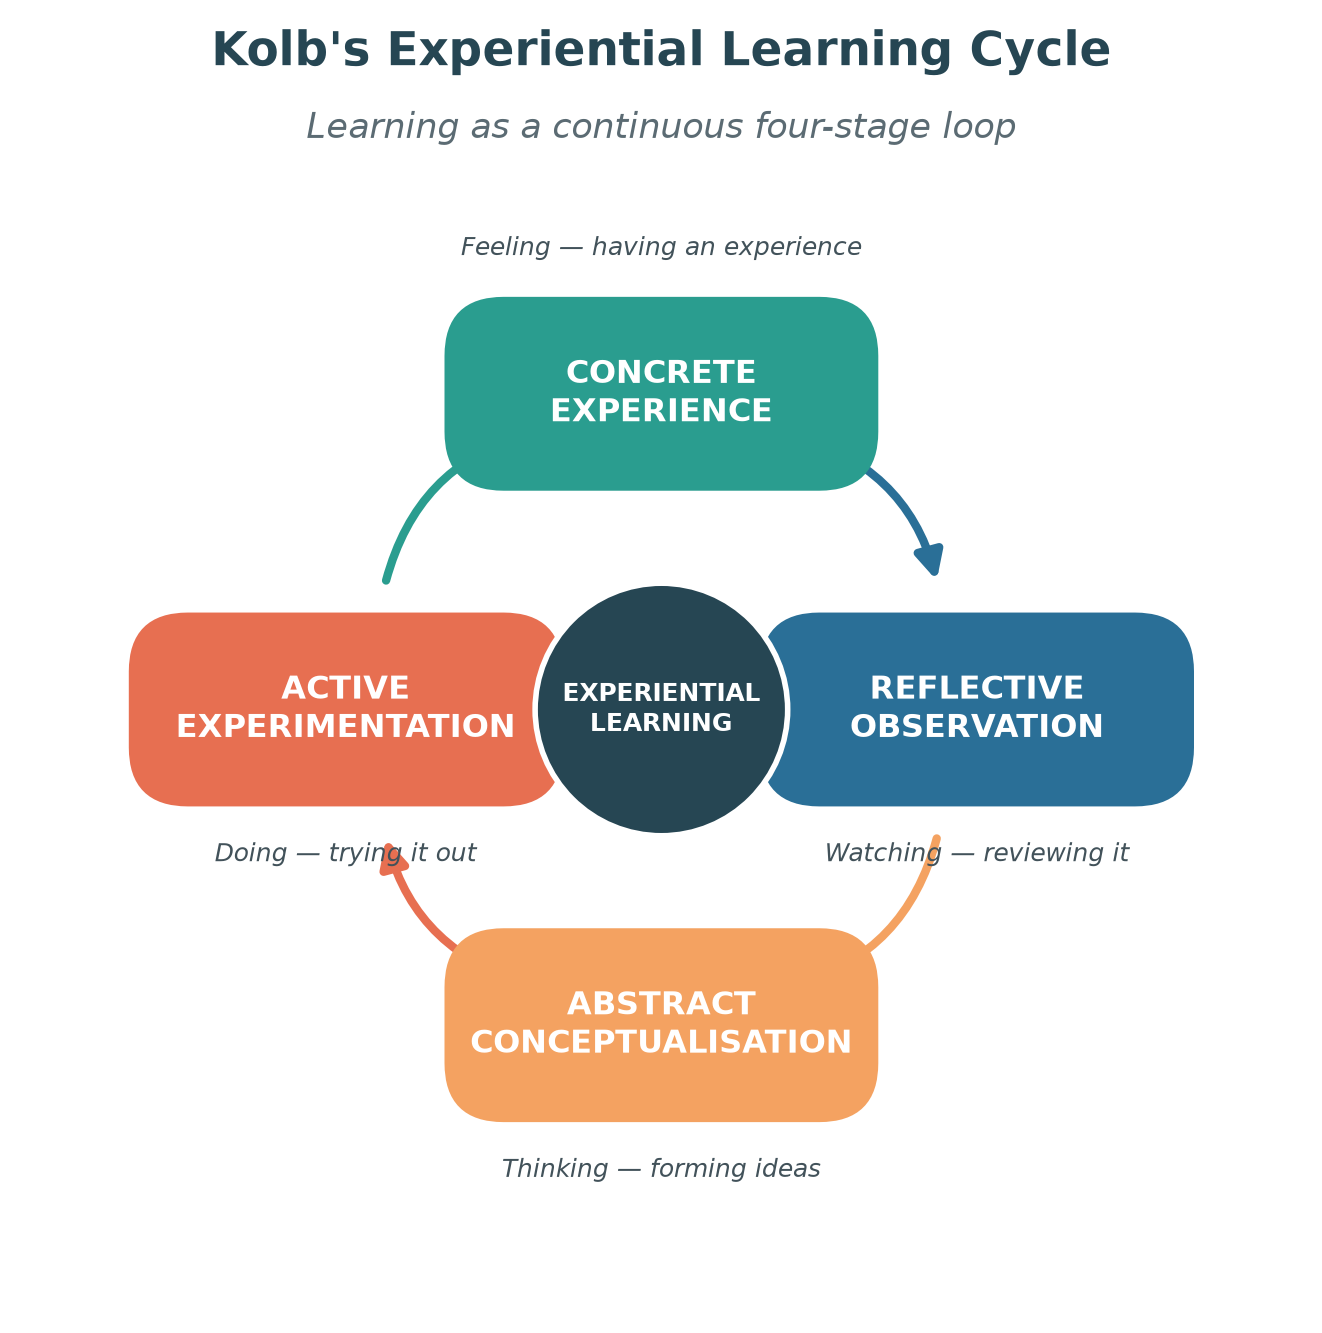
\includegraphics[width=\linewidth]{figures/kolb_cycle.png}
    \end{column}
    \begin{column}{0.45\textwidth}\footnotesize
      Learning is a \kw{continuous cycle} of four stages:
      \begin{enumerate}\footnotesize
        \item \kwt{Concrete Experience} — do / feel.
        \item \kwt{Reflective Observation} — review.
        \item \kwt{Abstract Conceptualisation} — conclude.
        \item \kwt{Active Experimentation} — plan \& try.
      \end{enumerate}
      Effective learning happens when we travel \emph{all the way round} the
      loop — repeatedly.
    \end{column}
  \end{columns}
\end{frame}

\begin{frame}{Kolb's Four Learning Styles}
  \begin{columns}[c]
    \begin{column}{0.58\textwidth}
      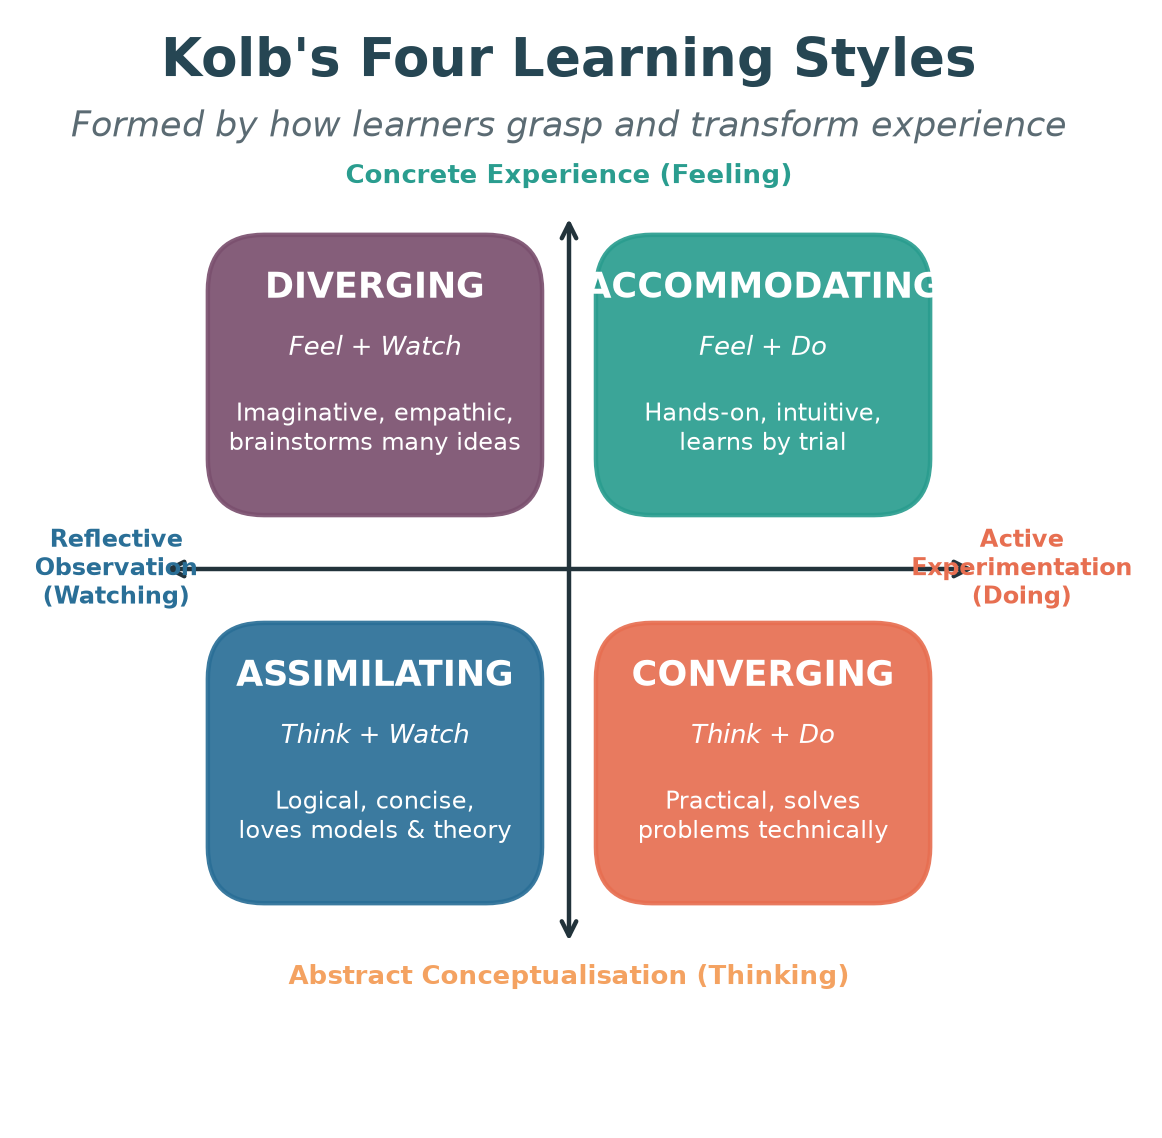
\includegraphics[width=\linewidth]{figures/kolb_styles.png}
    \end{column}
    \begin{column}{0.42\textwidth}\scriptsize
      Combining \emph{how we grasp} and \emph{how we transform} experience
      gives four styles:
      \begin{itemize}\scriptsize
        \item \pill{dtplum}{Diverging} — imaginative, many ideas.
        \item \pill{dtteal}{Accommodating} — hands-on, intuitive.
        \item \pill{dtblue}{Assimilating} — logical, loves theory.
        \item \pill{dtcoral}{Converging} — practical problem-solver.
      \end{itemize}
      \vspace{0.3em}
      Teams work best when \emph{all four styles} are present.
    \end{column}
  \end{columns}
\end{frame}

\begin{frame}{Assessing \& Interpreting Learning Styles}
  \accentrule\\[0.3em]
  \begin{columns}[T]
    \begin{column}{0.5\textwidth}\small
      \textbf{How we assess}
      \begin{itemize}\small
        \item \kw{Learning Style Inventory (LSI)} questionnaires.
        \item Self-reflection journals.
        \item Observation of behaviour in tasks.
      \end{itemize}
    \end{column}
    \begin{column}{0.5\textwidth}\small
      \textbf{How we interpret}
      \begin{itemize}\small
        \item No style is \emph{better} — each has strengths.
        \item Match \kwt{teaching methods} to styles.
        \item Encourage learners to stretch into weaker modes.
      \end{itemize}
    \end{column}
  \end{columns}
  \vspace{0.4em}
  \begin{block}{Application with peers}
    \scriptsize In group projects, deliberately mix styles so ideation,
    analysis, building and testing are all covered.
  \end{block}
\end{frame}

\begin{frame}{The Memory Process}
  \bigfig{memory_process.png}{The information-processing model: sensory $\to$ short-term $\to$ long-term memory.}
\end{frame}

\begin{frame}{Problems in Retention}
  \accentrule\\[0.3em]
  \begin{columns}[T]
    \begin{column}{0.5\textwidth}\small
      Why do we forget?
      \begin{itemize}\small
        \item \kwc{Decay} — traces fade without use.
        \item \kwc{Interference} — old \& new memories clash.
        \item \kwc{Retrieval failure} — no cue to recall.
        \item \kwc{Weak encoding} — shallow processing.
      \end{itemize}
    \end{column}
    \begin{column}{0.5\textwidth}
      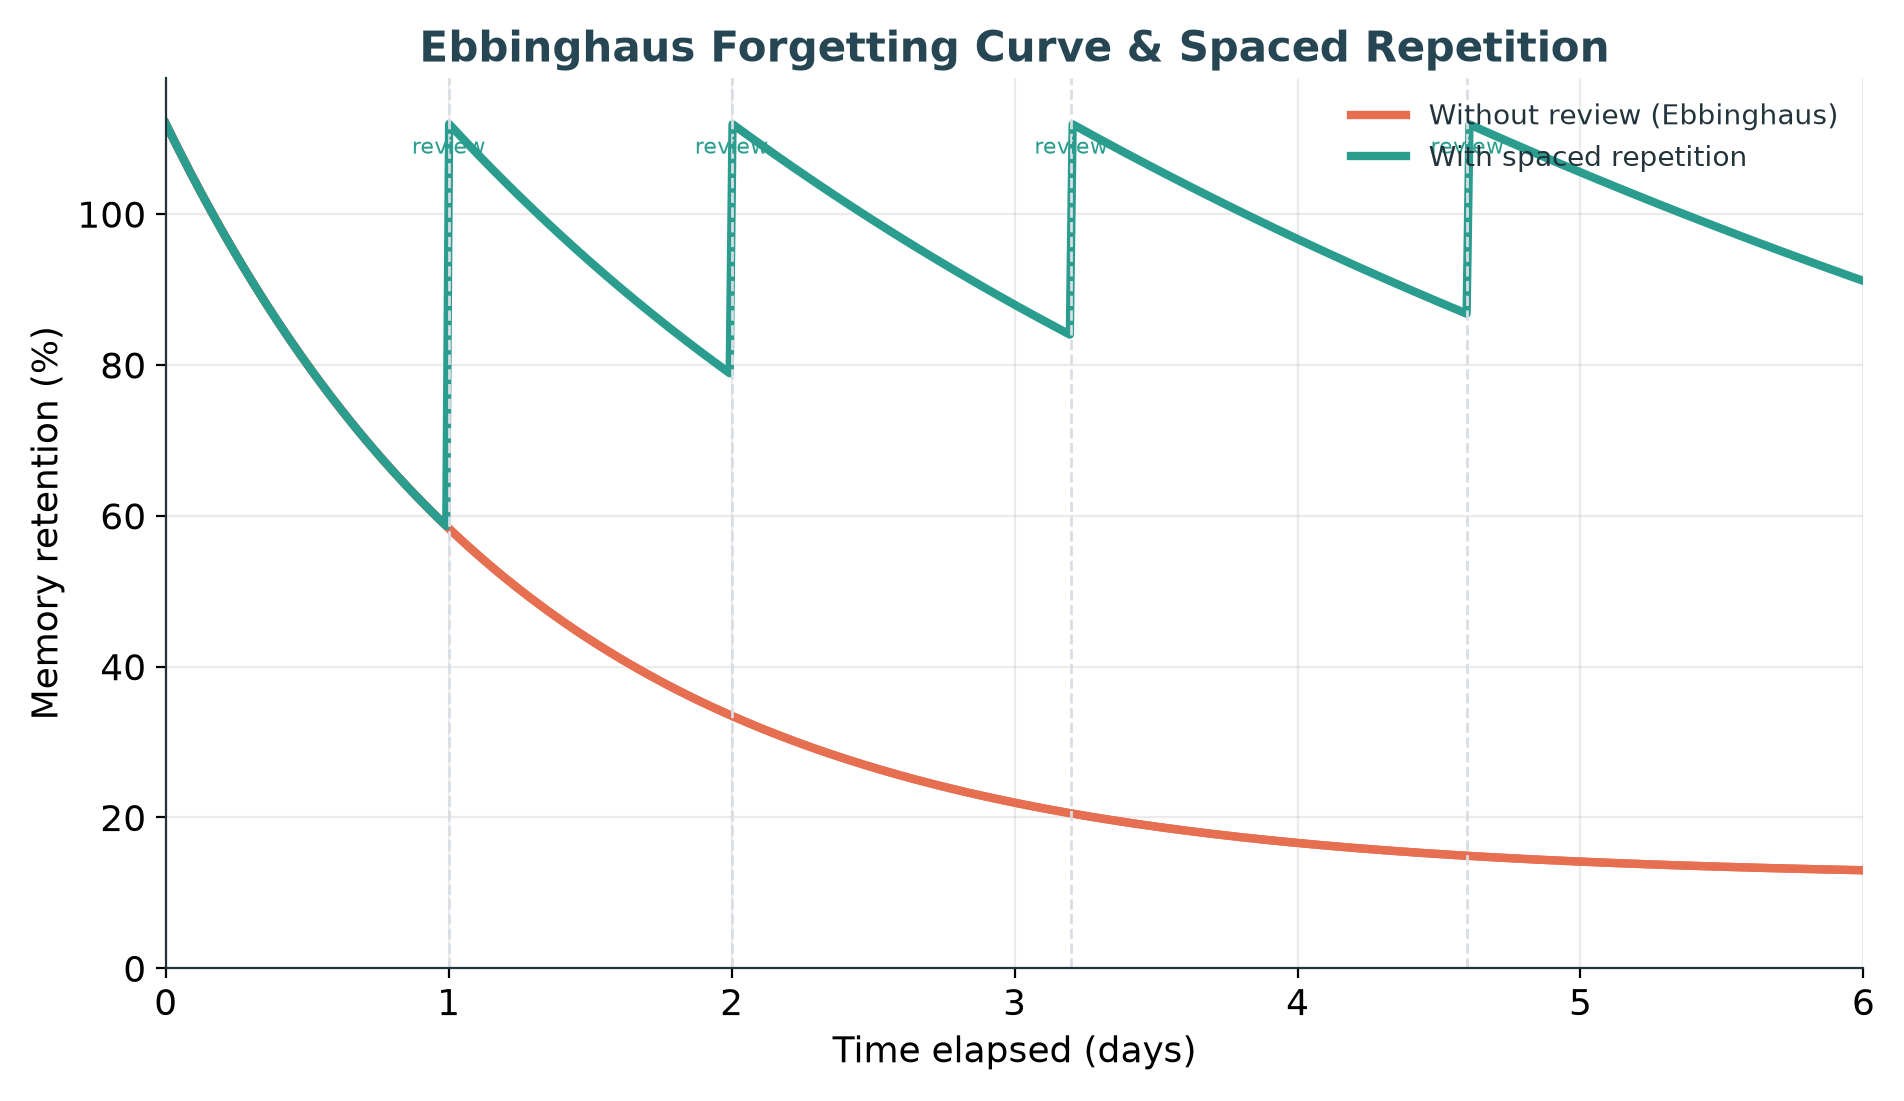
\includegraphics[width=\linewidth]{figures/forgetting_curve.png}
    \end{column}
  \end{columns}
  \vspace{0.2em}
  {\scriptsize The \kw{Ebbinghaus curve} shows rapid forgetting — but each
  review flattens the curve.}
\end{frame}

\begin{frame}{Memory Enhancement Techniques}
  \accentrule\\[0.4em]
  \begin{columns}[T]
    \begin{column}{0.5\textwidth}\small
      \begin{itemize}\small
        \item \kwt{Chunking} — group items into meaningful units.
        \item \kwt{Mnemonics} — acronyms, rhymes, imagery.
        \item \kwt{Spaced repetition} — review at intervals.
        \item \kwt{Elaboration} — connect to prior knowledge.
      \end{itemize}
    \end{column}
    \begin{column}{0.5\textwidth}\small
      \begin{itemize}\small
        \item \kwt{Dual coding} — words + visuals together.
        \item \kwt{Active recall} — test yourself, don't re-read.
        \item \kwt{Method of loci} — memory "palace".
        \item \kwt{Sleep \& rest} — consolidate memories.
      \end{itemize}
    \end{column}
  \end{columns}
  \vspace{0.4em}
  \begin{block}{Design tip}\scriptsize
    Good product design \emph{reduces the memory load} on the user — clear
    labels, consistent layouts and helpful cues.
  \end{block}
\end{frame}

\begin{frame}{Emotions, Experience \& Expression}
  \accentrule\\[0.3em]
  \begin{columns}[T]
    \begin{column}{0.55\textwidth}\small
      Emotions shape how people \kw{experience} and \kw{remember} products.
      \begin{itemize}\small
        \item \kwt{Emotion} — an internal feeling (joy, frustration, trust).
        \item \kwt{Experience} — the felt journey of using something.
        \item \kwt{Expression} — how emotion is shown \& communicated.
      \end{itemize}
      \vspace{0.3em}
      Peak emotions (delight or annoyance) leave the strongest memories —
      the \emph{peak-end rule}.
    \end{column}
    \begin{column}{0.45\textwidth}
      \begin{block}{Emotional design (Norman)}\scriptsize
        \begin{itemize}\scriptsize
          \item \textbf{Visceral} — first look \& feel.
          \item \textbf{Behavioural} — pleasure of use.
          \item \textbf{Reflective} — meaning \& self-image.
        \end{itemize}
      \end{block}
    \end{column}
  \end{columns}
\end{frame}

\begin{frame}{Empathy \& Emotional Intelligence}
  \begin{columns}[c]
    \begin{column}{0.6\textwidth}
      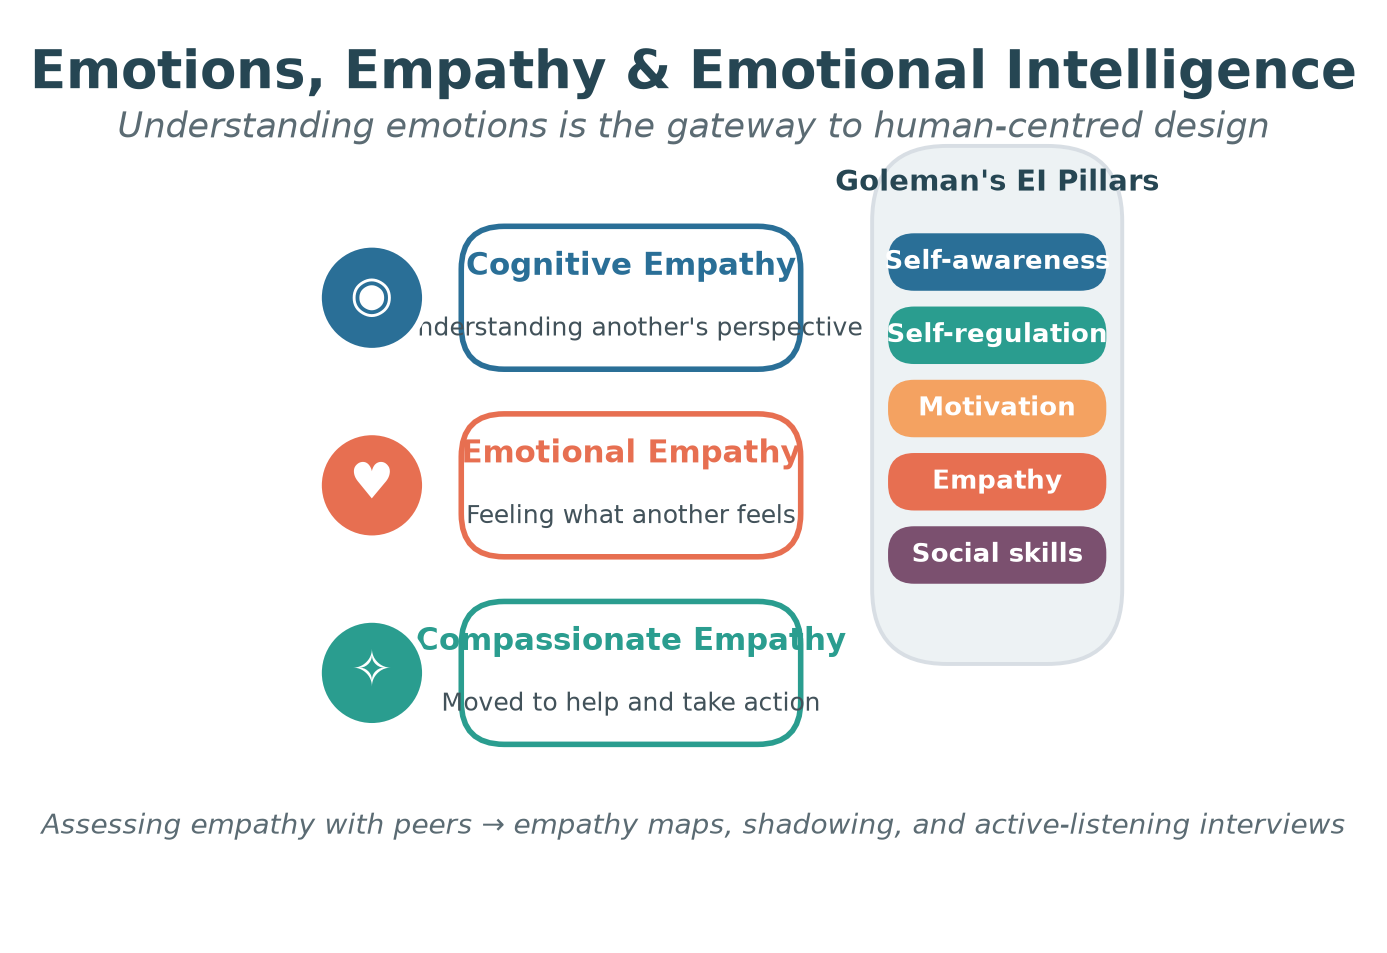
\includegraphics[width=\linewidth]{figures/empathy.png}
    \end{column}
    \begin{column}{0.4\textwidth}\scriptsize
      \kw{Empathy} — the ability to understand and share another's feelings —
      is the \emph{heart of design thinking}.
      \vspace{0.3em}
      \textbf{Assessing empathy with peers}
      \begin{itemize}\scriptsize
        \item Empathy maps (says / thinks / does / feels).
        \item Shadowing \& observation.
        \item Active-listening interviews.
      \end{itemize}
    \end{column}
  \end{columns}
\end{frame}

%==============================================================================
\section{Basics of Design Thinking}
%==============================================================================
\unitdivider{II}{Basics of Design Thinking}{The mindset, the process, the tools}

\begin{frame}{What is Design Thinking?}
  \accentrule\\[0.3em]
  \begin{columns}[T]
    \begin{column}{0.55\textwidth}\small
      \begin{block}{Definition}\small
        A \kw{human-centred}, iterative problem-solving approach that seeks
        to understand users, challenge assumptions, redefine problems and
        create innovative solutions to prototype and test.
      \end{block}
      \textbf{Need for design thinking}
      \begin{itemize}\small
        \item Problems are \kwc{complex \& ill-defined}.
        \item Users' real needs are often \emph{hidden}.
        \item Reduces the risk of building the wrong thing.
      \end{itemize}
    \end{column}
    \begin{column}{0.45\textwidth}\small
      \textbf{Objectives}
      \begin{itemize}\small
        \item Keep the \kwt{user at the centre}.
        \item Encourage \kwt{creativity \& collaboration}.
        \item \kwt{Fail early}, learn cheaply.
        \item Turn insight into tangible value.
      \end{itemize}
    \end{column}
  \end{columns}
\end{frame}

\begin{frame}{Concepts \& Brainstorming}
  \begin{columns}[c]
    \begin{column}{0.58\textwidth}
      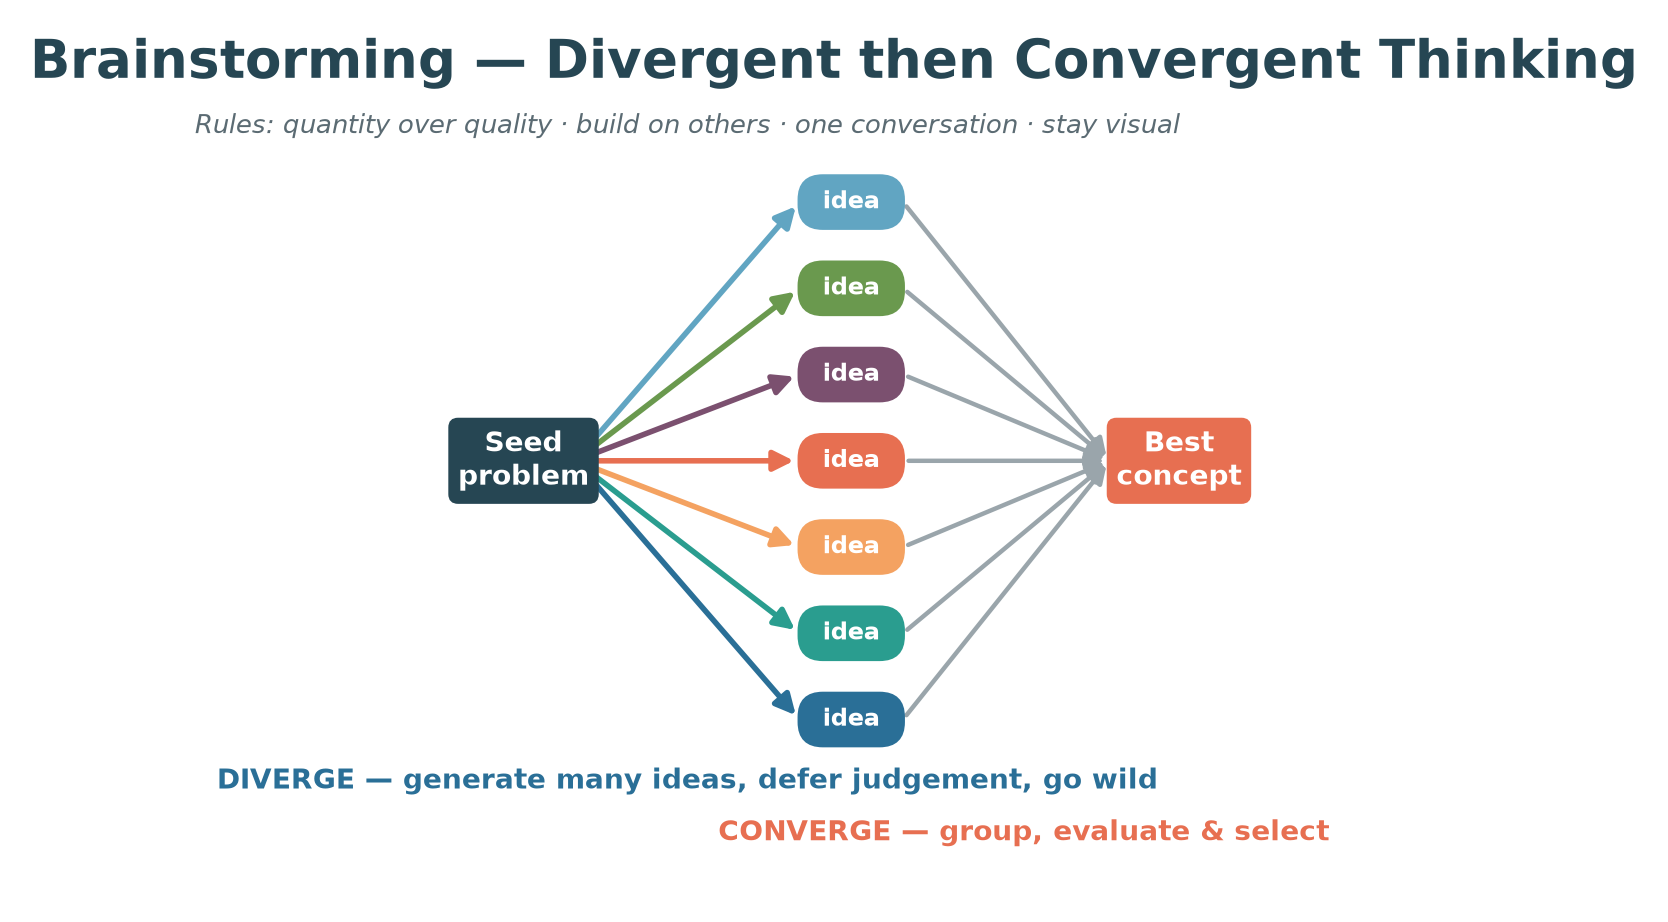
\includegraphics[width=\linewidth]{figures/divergent_convergent.png}
    \end{column}
    \begin{column}{0.42\textwidth}\scriptsize
      Creative work alternates two modes:
      \begin{itemize}\scriptsize
        \item \pill{dtblue}{Diverge} — generate many ideas, defer judgement.
        \item \pill{dtcoral}{Converge} — group, evaluate \& select.
      \end{itemize}
      \vspace{0.3em}
      \textbf{Brainstorming rules}
      \begin{itemize}\scriptsize
        \item Go for quantity.
        \item Build on others' ideas.
        \item One conversation at a time.
        \item Stay visual; welcome wild ideas.
      \end{itemize}
    \end{column}
  \end{columns}
\end{frame}

\begin{frame}{The Five Stages of Design Thinking}
  \bigfig{dt_process.png}{Empathize $\to$ Define $\to$ Ideate $\to$ Prototype $\to$ Test — iterative, not linear.}
\end{frame}

\begin{frame}{Stages in Detail (1--3)}
  \accentrule\\[0.3em]
  \small
  \begin{description}\small
    \item[\textcolor{dtblue}{1. Empathize}] Observe and engage with users;
      conduct interviews and immerse yourself in their world. \emph{Example:}
      shadowing commuters to learn how they use a ticket machine.
    \item[\textcolor{dtteal}{2. Define}] Synthesise observations into a clear,
      user-centred \kw{problem statement} (a Point-of-View). \emph{Example:}
      "Busy commuters need a faster way to buy tickets because queues cause
      stress."
    \item[\textcolor{dtyellow}{3. Ideate}] Generate a wide range of ideas
      through brainstorming, sketching and mind-mapping — \emph{quantity over
      quality} first.
  \end{description}
\end{frame}

\begin{frame}{Stages in Detail (4--5)}
  \accentrule\\[0.3em]
  \small
  \begin{description}\small
    \item[\textcolor{dtorange}{4. Prototype}] Build quick, inexpensive,
      scaled-down versions to explore ideas. \emph{Example:} a paper mock-up of
      the ticket-machine screen.
    \item[\textcolor{dtcoral}{5. Test}] Try prototypes with real users, gather
      feedback and refine. Testing often \emph{re-defines the problem} —
      sending you back to earlier stages.
  \end{description}
  \vspace{0.3em}
  \begin{block}{Being ingenious}\scriptsize
    The stages are a \emph{flexible toolkit}, not a rigid recipe. Teams loop,
    skip and revisit stages as they learn.
  \end{block}
\end{frame}

\begin{frame}{The Double Diamond}
  \begin{columns}[c]
    \begin{column}{0.62\textwidth}
      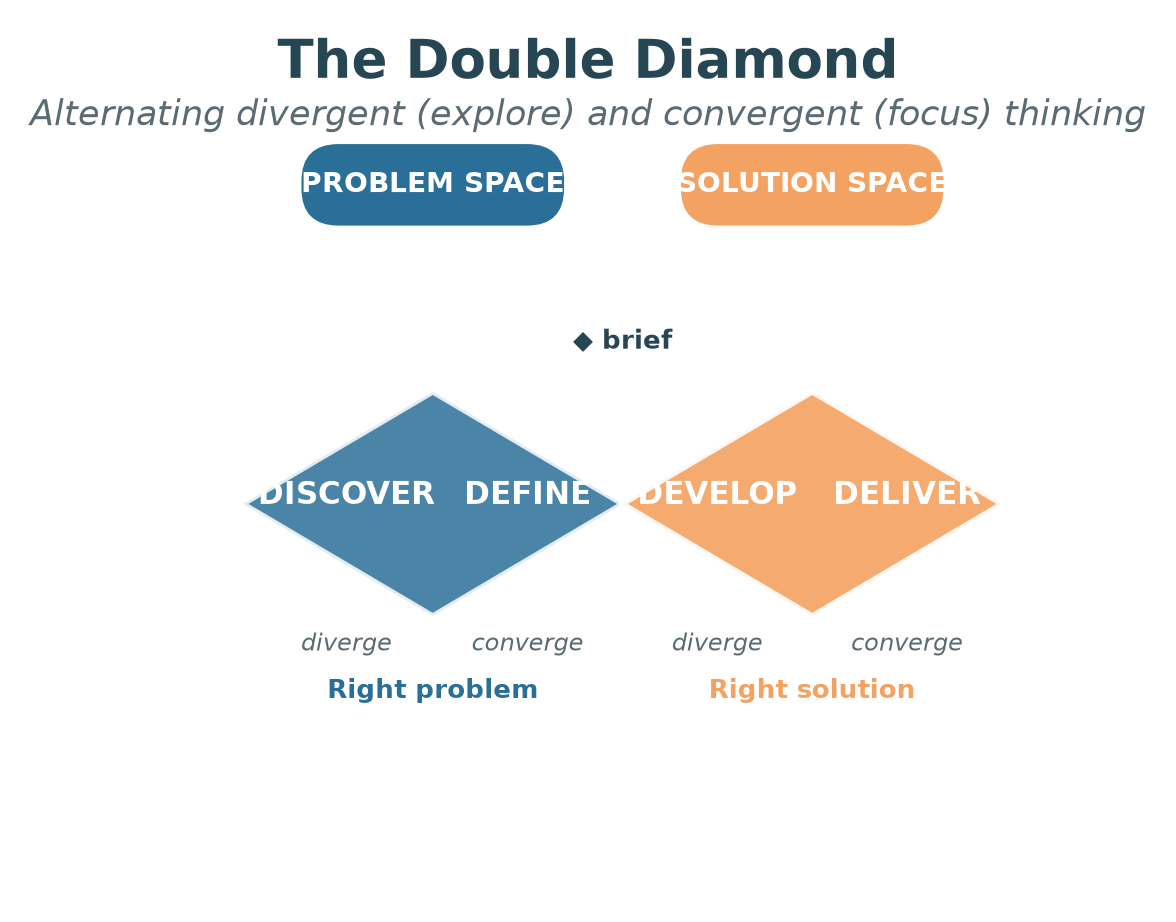
\includegraphics[width=\linewidth]{figures/double_diamond.png}
    \end{column}
    \begin{column}{0.38\textwidth}\scriptsize
      A popular map of the design process:
      \begin{itemize}\scriptsize
        \item \pill{dtblue}{Discover \& Define} — find the \emph{right problem}.
        \item \pill{dtorange}{Develop \& Deliver} — build the \emph{right
              solution}.
      \end{itemize}
      \vspace{0.3em}
      Each diamond widens (diverge) then narrows (converge).
    \end{column}
  \end{columns}
\end{frame}

\begin{frame}{Creative Thinking \& Problem Solving}
  \begin{columns}[c]
    \begin{column}{0.6\textwidth}
      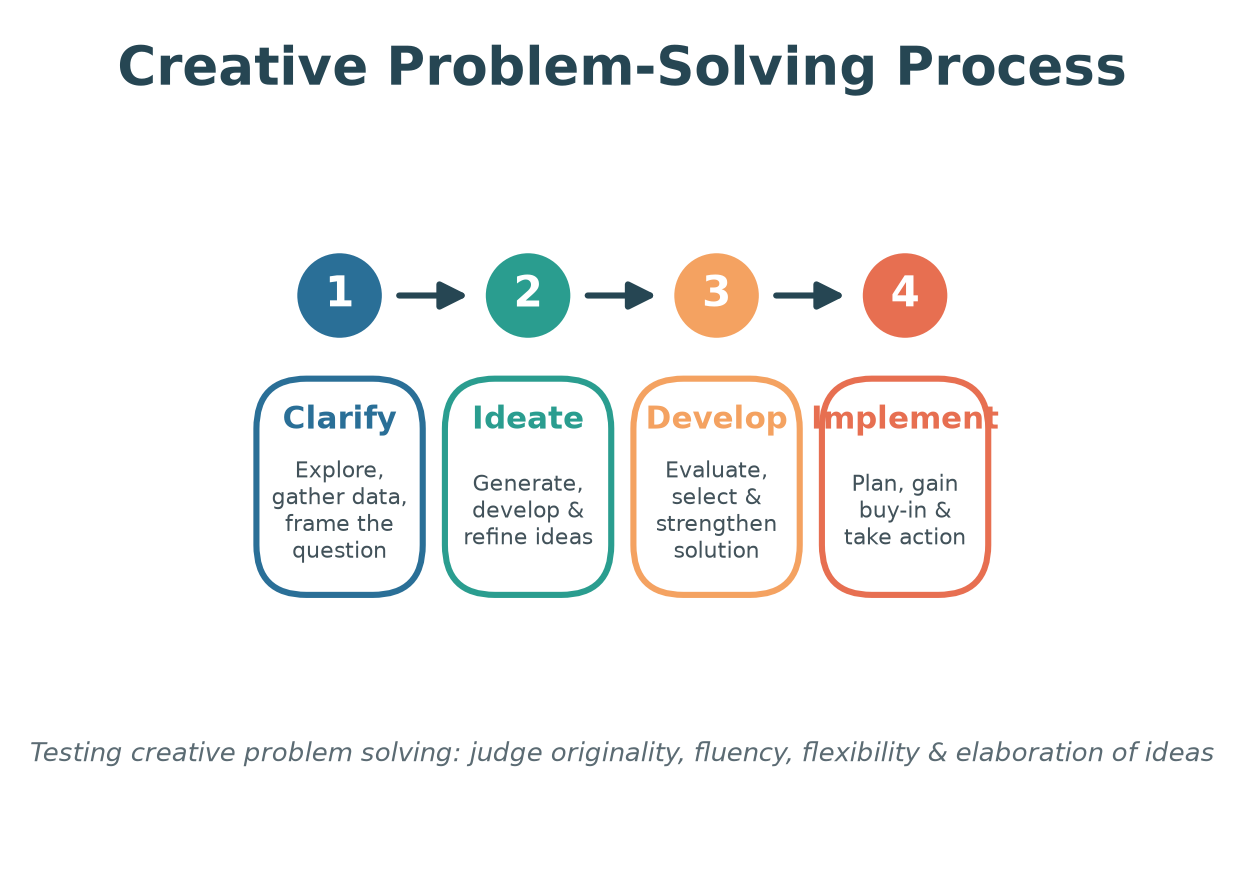
\includegraphics[width=\linewidth]{figures/creative_problem_solving.png}
    \end{column}
    \begin{column}{0.4\textwidth}\scriptsize
      Creative problem solving moves through four stages: \kwt{Clarify},
      \kwt{Ideate}, \kwt{Develop} and \kwt{Implement}.
      \vspace{0.4em}
      \textbf{Testing creative problem solving} — judge ideas on:
      \begin{itemize}\scriptsize
        \item \emph{Fluency} — number of ideas.
        \item \emph{Flexibility} — variety of ideas.
        \item \emph{Originality} — novelty.
        \item \emph{Elaboration} — detail \& refinement.
      \end{itemize}
    \end{column}
  \end{columns}
\end{frame}

%==============================================================================
\section{Process of Product Design}
%==============================================================================
\unitdivider{III}{Process of Product Design}{Engineering design, prototyping \& testing}

\begin{frame}{Engineering Product-Design Process}
  \bigfig{product_design_process.png}{A structured flow from identifying a need to manufacture \& launch.}
\end{frame}

\begin{frame}{Design-Thinking Approach to Product Design}
  \accentrule\\[0.3em]
  \begin{columns}[T]
    \begin{column}{0.5\textwidth}\small
      \textbf{Traditional engineering}
      \begin{itemize}\small
        \item Requirements defined up front.
        \item Linear, specification-driven.
        \item User feedback comes late.
      \end{itemize}
    \end{column}
    \begin{column}{0.5\textwidth}\small
      \textbf{Design-thinking infused}
      \begin{itemize}\small
        \item \kwt{User needs} continuously explored.
        \item \kwt{Iterative} — prototype \& test early.
        \item Feedback loops at \emph{every} stage.
      \end{itemize}
    \end{column}
  \end{columns}
  \vspace{0.3em}
  \begin{block}{Best in class}\scriptsize
    Great products (e.g.\ intuitive smartphones, ergonomic tools,
    well-designed appliances) combine \emph{function}, \emph{form} and
    \emph{delight} — form follows function \emph{and} feeling.
  \end{block}
\end{frame}

\begin{frame}{What is a Prototype?}
  \accentrule\\[0.3em]
  \begin{columns}[T]
    \begin{column}{0.52\textwidth}\small
      A \kw{prototype} is an early, testable model of a product used to
      \emph{explore ideas} and \emph{learn} before committing to production.
      \vspace{0.3em}
      \textbf{Why prototype?}
      \begin{itemize}\small
        \item Make ideas \kwt{tangible}.
        \item Test assumptions cheaply.
        \item Communicate with stakeholders.
        \item Fail fast, improve faster.
      \end{itemize}
    \end{column}
    \begin{column}{0.48\textwidth}\small
      \textbf{Types of prototype}
      \begin{itemize}\small
        \item \emph{Low-fidelity} — sketches, paper, cardboard.
        \item \emph{Mid-fidelity} — wireframes, models.
        \item \emph{High-fidelity} — 3-D printed, functional.
      \end{itemize}
    \end{column}
  \end{columns}
\end{frame}

\begin{frame}{Prototype Fidelity Ladder}
  \begin{columns}[c]
    \begin{column}{0.6\textwidth}
      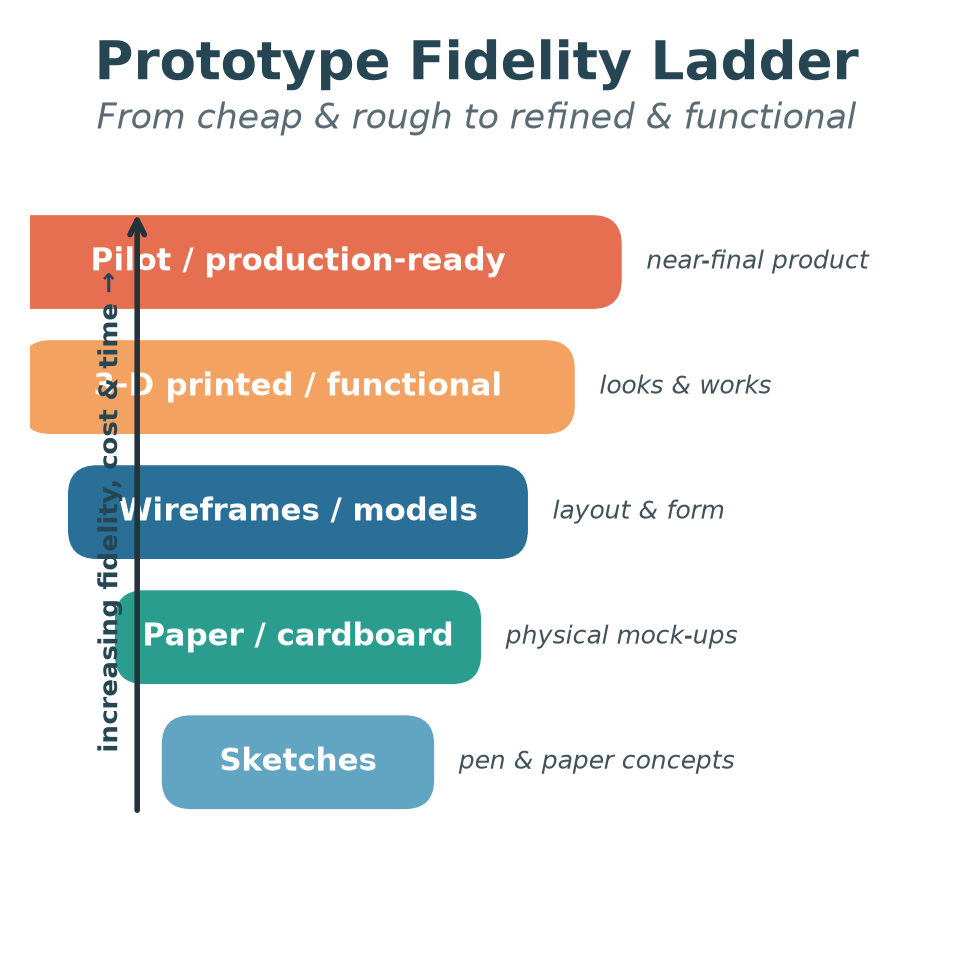
\includegraphics[width=\linewidth]{figures/prototype_fidelity.png}
    \end{column}
    \begin{column}{0.4\textwidth}\scriptsize
      Start \kwt{low} and cheap, climb only as questions demand.
      \vspace{0.3em}
      \begin{itemize}\scriptsize
        \item Low fidelity answers \emph{"is this the right idea?"}
        \item High fidelity answers \emph{"does it work \& feel right?"}
      \end{itemize}
      \vspace{0.3em}
      Each rung costs more time and money — so \emph{learn cheaply first}.
    \end{column}
  \end{columns}
\end{frame}

\begin{frame}{Rapid Prototype Development}
  \begin{columns}[c]
    \begin{column}{0.55\textwidth}
      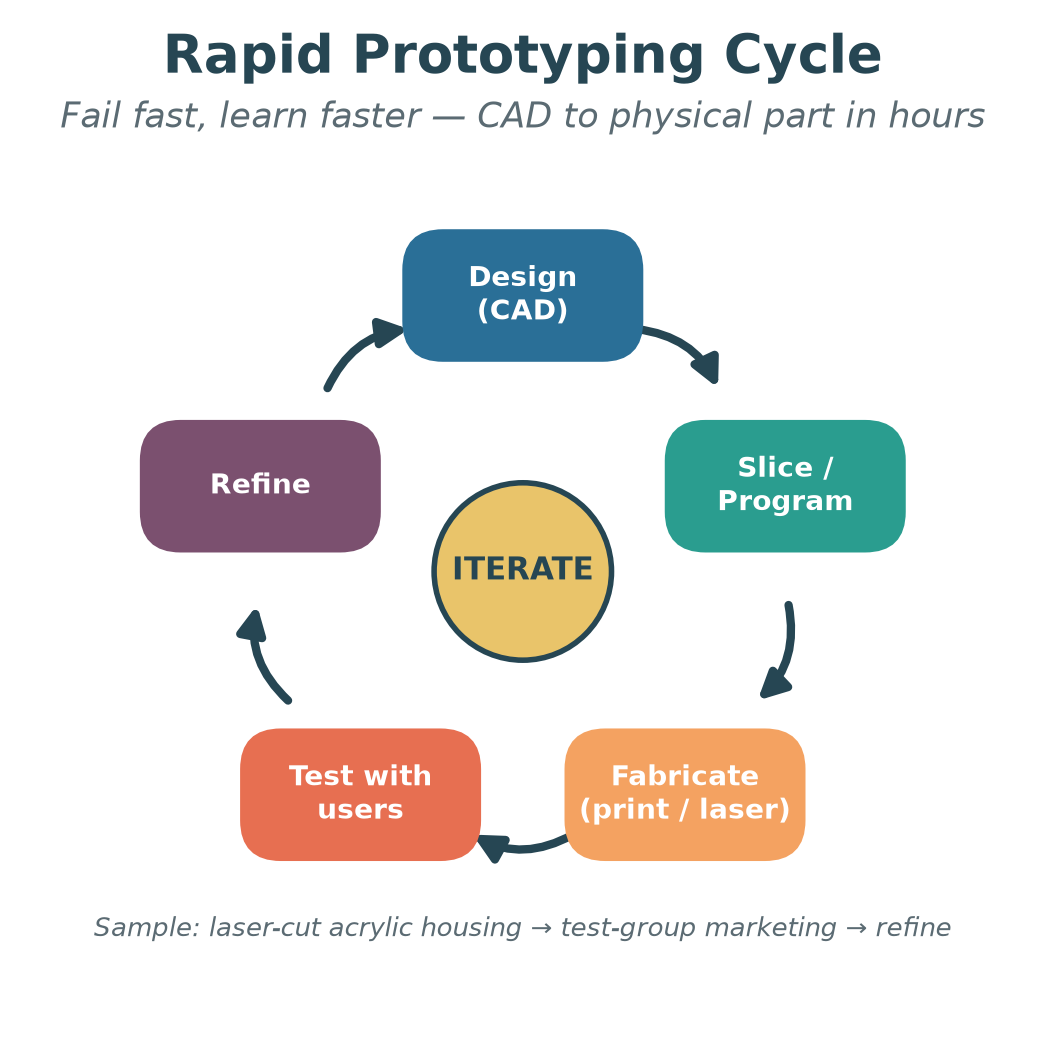
\includegraphics[width=\linewidth]{figures/rapid_prototyping.png}
    \end{column}
    \begin{column}{0.45\textwidth}\scriptsize
      \kw{Rapid prototyping} uses digital fabrication (3-D printing, laser
      cutting, CNC) to go from \kwt{CAD} to a physical part in \emph{hours}.
      \vspace{0.3em}
      \textbf{Testing \& sample marketing}
      \begin{itemize}\scriptsize
        \item Test the prototype with a small \kwt{test group}.
        \item Gather reactions before scaling up.
        \item Refine, then repeat the loop.
      \end{itemize}
    \end{column}
  \end{columns}
\end{frame}

%==============================================================================
\section{Design Thinking \& Customer Centricity}
%==============================================================================
\unitdivider{IV}{Design Thinking \&\\Customer Centricity}{Experience, feedback \& re-creation}

\begin{frame}{Practical Customer Challenges}
  \accentrule\\[0.3em]
  \small
  Real customers face everyday frustrations that design thinking can solve:
  \begin{columns}[T]
    \begin{column}{0.5\textwidth}
      \begin{itemize}\small
        \item Products that are \kwc{hard to assemble} or use.
        \item Confusing instructions \& interfaces.
        \item Poor \kwc{ergonomics} causing discomfort.
      \end{itemize}
    \end{column}
    \begin{column}{0.5\textwidth}
      \begin{itemize}\small
        \item Long waits and clunky service.
        \item Features nobody asked for.
        \item A gap between the \emph{promise} and the \emph{experience}.
      \end{itemize}
    \end{column}
  \end{columns}
  \vspace{0.4em}
  \begin{block}{Design thinking to the rescue}\scriptsize
    By empathising with customers we uncover these pains and re-design the
    product experience around them.
  \end{block}
\end{frame}

\begin{frame}{Parameters of Product Experience}
  \begin{columns}[c]
    \begin{column}{0.55\textwidth}
      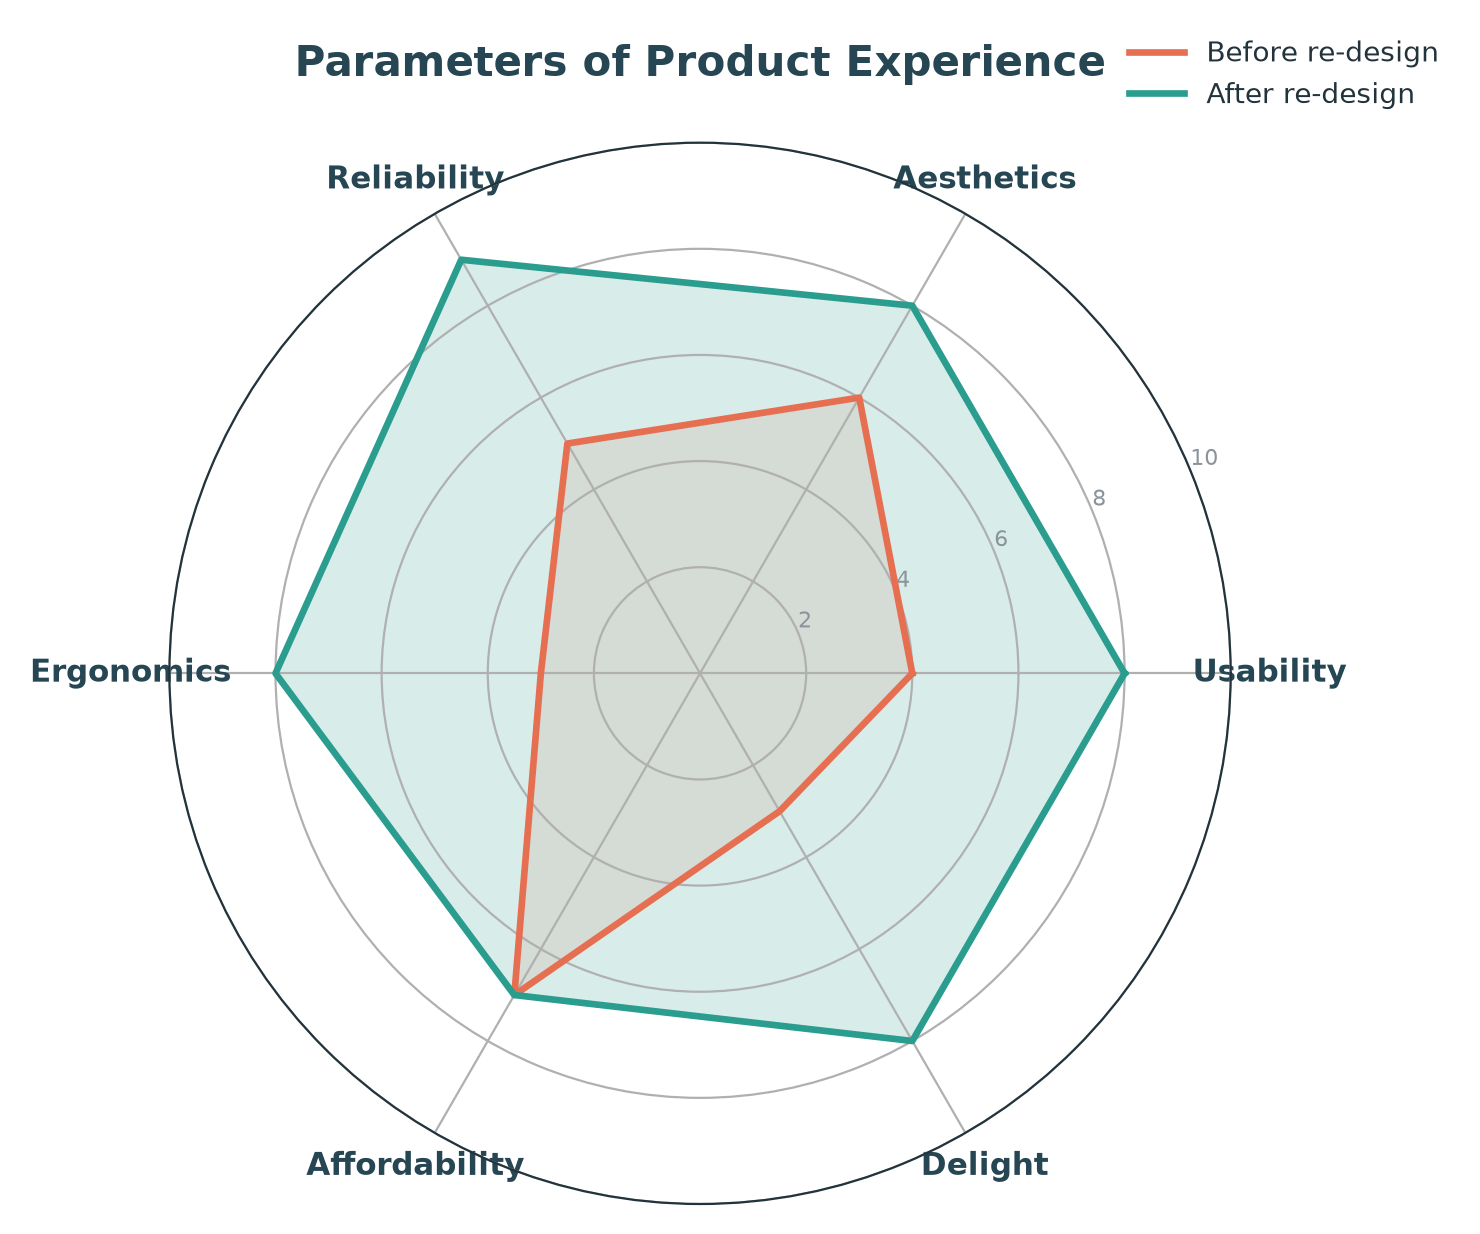
\includegraphics[width=\linewidth]{figures/cx_radar.png}
    \end{column}
    \begin{column}{0.45\textwidth}\scriptsize
      Product experience is multi-dimensional:
      \begin{itemize}\scriptsize
        \item \kwt{Usability} \& \kwt{Reliability}
        \item \kwt{Aesthetics} \& \kwt{Ergonomics}
        \item \kwt{Affordability} \& \kwt{Delight}
      \end{itemize}
      \vspace{0.3em}
      Thoughtful re-design lifts every axis — turning a merely functional
      product into one customers \emph{love}.
    \end{column}
  \end{columns}
\end{frame}

\begin{frame}{Aligning Customer Expectations}
  \begin{columns}[c]
    \begin{column}{0.55\textwidth}
      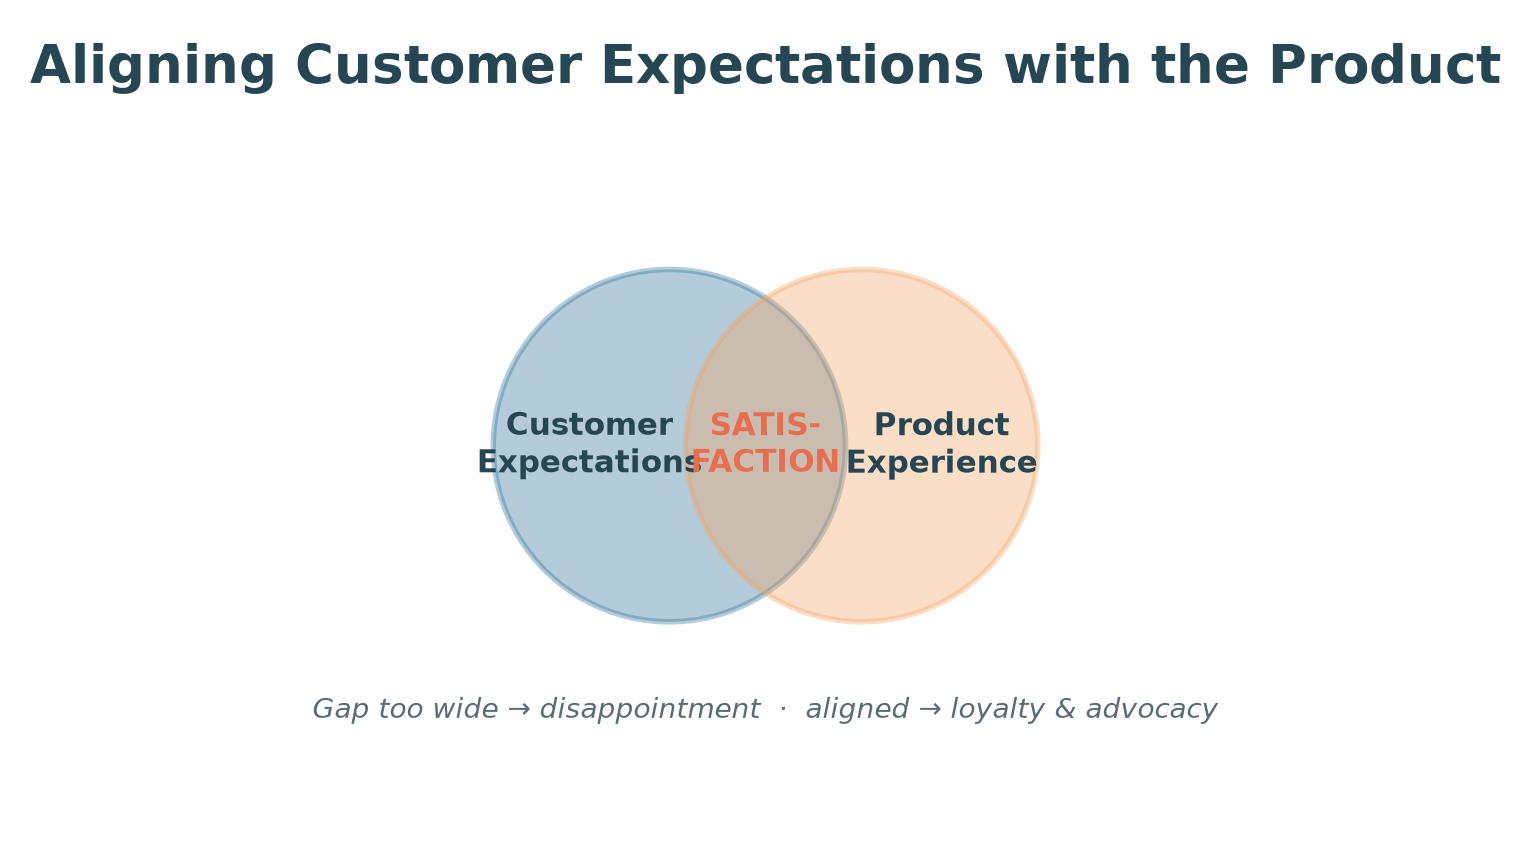
\includegraphics[width=\linewidth]{figures/expectation_alignment.png}
    \end{column}
    \begin{column}{0.45\textwidth}\scriptsize
      \kw{Satisfaction} lives where \emph{expectations} meet \emph{experience}.
      \begin{itemize}\scriptsize
        \item Gap too wide $\to$ disappointment.
        \item Well aligned $\to$ loyalty \& advocacy.
      \end{itemize}
      \vspace{0.3em}
      Manage expectations honestly \emph{and} raise the experience to close
      the gap.
    \end{column}
  \end{columns}
\end{frame}

\begin{frame}{Feedback, Re-Design \& Re-Create}
  \begin{columns}[c]
    \begin{column}{0.52\textwidth}
      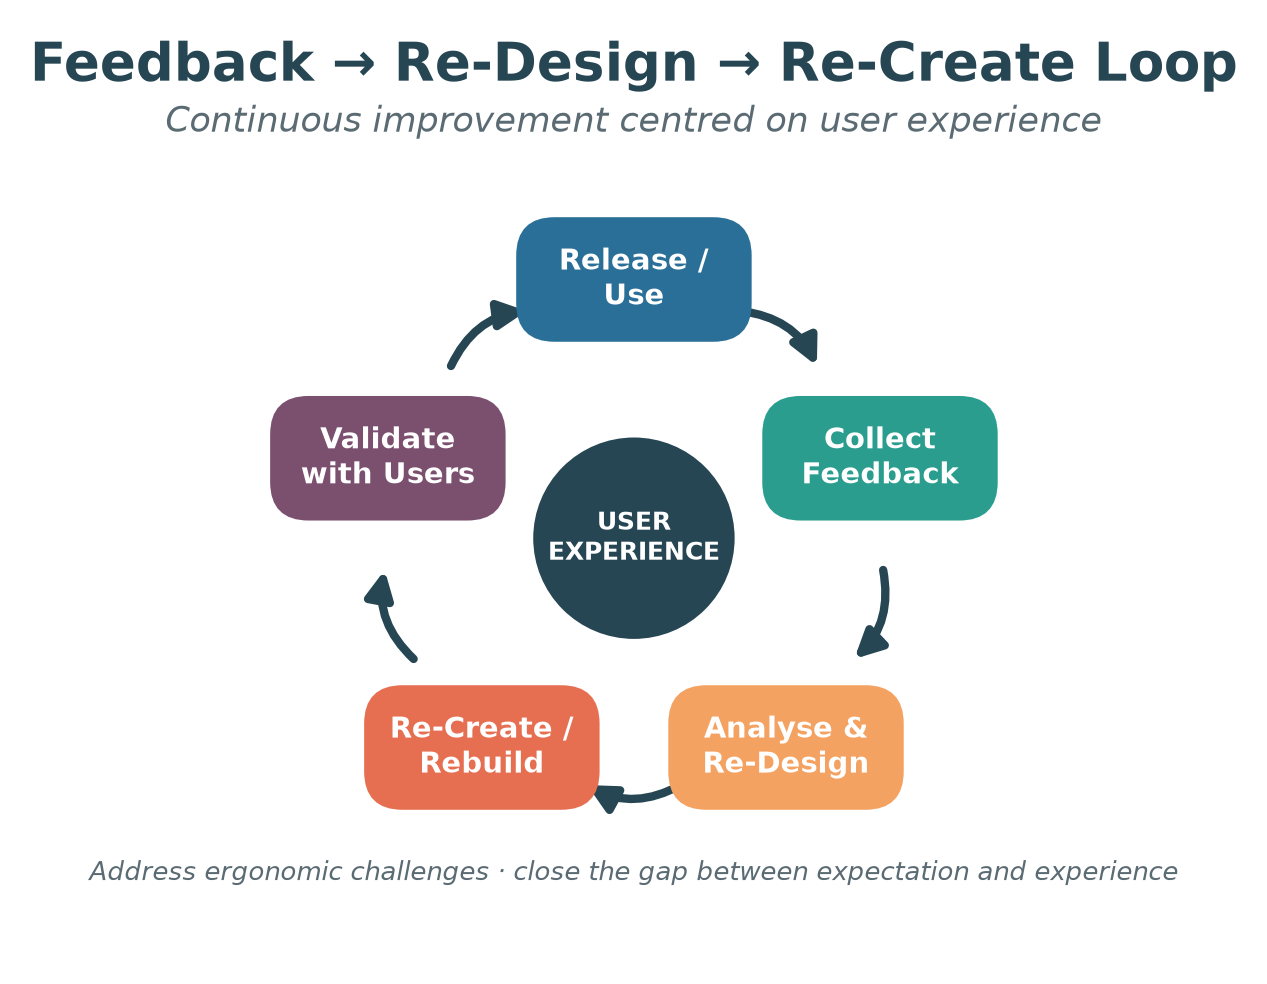
\includegraphics[width=\linewidth]{figures/feedback_loop.png}
    \end{column}
    \begin{column}{0.48\textwidth}\scriptsize
      The \kw{feedback loop} keeps a product improving:
      \begin{enumerate}\scriptsize
        \item Release \& use.
        \item Collect feedback.
        \item Analyse \& re-design.
        \item Re-create / rebuild.
        \item Validate with users.
      \end{enumerate}
      \vspace{0.2em}
      Focus relentlessly on \kwt{user experience} and address ergonomic
      challenges each cycle.
    \end{column}
  \end{columns}
\end{frame}

\begin{frame}{User-Focused Design \& the Final Product}
  \accentrule\\[0.3em]
  \begin{columns}[T]
    \begin{column}{0.5\textwidth}\small
      \textbf{User-focused design}
      \begin{itemize}\small
        \item Design \emph{with} users, not just for them.
        \item Fit the product to the human — \kwt{ergonomics}.
        \item Test with real tasks in real contexts.
      \end{itemize}
    \end{column}
    \begin{column}{0.5\textwidth}\small
      \textbf{Toward the final product}
      \begin{itemize}\small
        \item Converge feedback into refinements.
        \item Validate safety, comfort \& usability.
        \item Ship — then keep listening.
      \end{itemize}
    \end{column}
  \end{columns}
  \vspace{0.3em}
  \begin{block}{Remember}\scriptsize
    A "final" product is really the \emph{best current version} — the loop
    never truly ends.
  \end{block}
\end{frame}

%==============================================================================
\section{Fabrication Laboratory}
%==============================================================================
\unitdivider{V}{Fabrication Laboratory}{The route map: survey to service blueprint}

\begin{frame}{The Fab-Lab Route Map}
  \begin{columns}[c]
    \begin{column}{0.5\textwidth}
      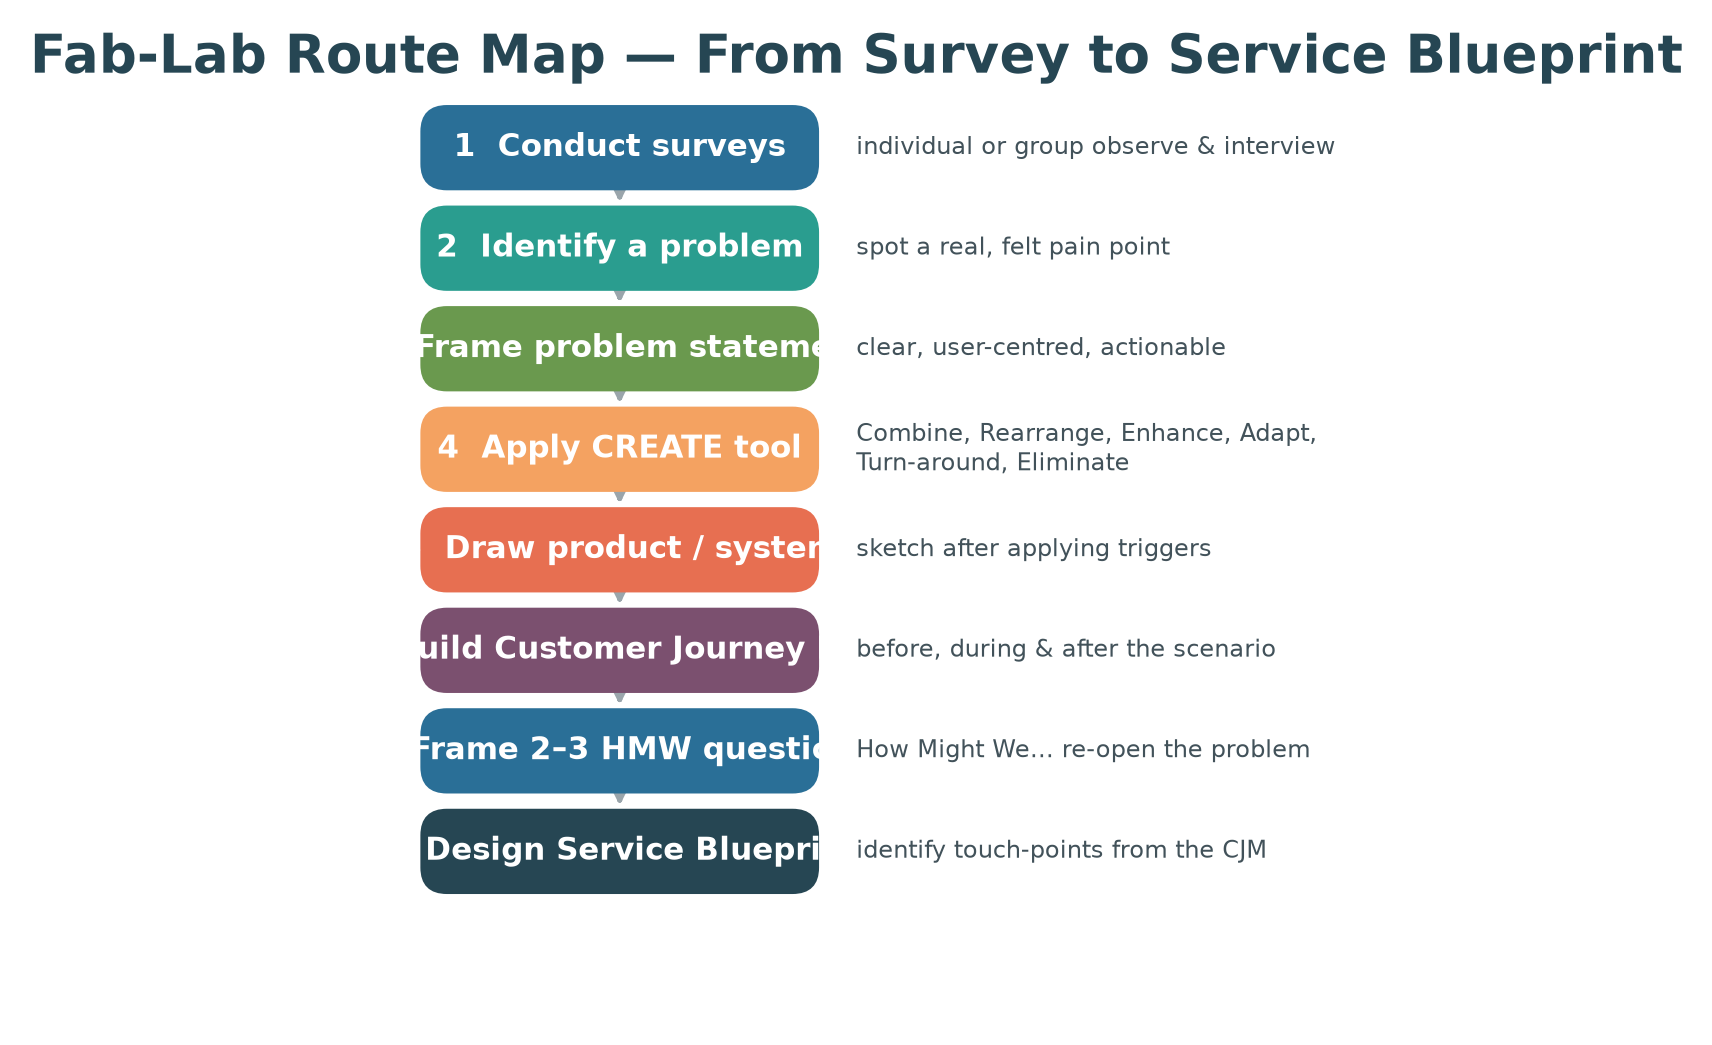
\includegraphics[width=\linewidth]{figures/route_map.png}
    \end{column}
    \begin{column}{0.5\textwidth}\scriptsize
      A step-by-step recipe for the lab project:
      \begin{enumerate}\scriptsize
        \item Conduct surveys.
        \item Identify a problem.
        \item Frame a problem statement.
        \item Apply the \kwt{CREATE} tool.
        \item Draw the product / system.
        \item Build a Customer Journey Map.
        \item Frame 2--3 \kwt{HMW} questions.
        \item Design a Service Blueprint.
      \end{enumerate}
    \end{column}
  \end{columns}
\end{frame}

\begin{frame}{Surveys, Problems \& Problem Statements}
  \accentrule\\[0.3em]
  \begin{columns}[T]
    \begin{column}{0.5\textwidth}\small
      \textbf{Conduct surveys}
      \begin{itemize}\small
        \item Individually or as a group.
        \item Observe, interview, question.
        \item Look for \kwc{real, felt pains}.
      \end{itemize}
      \textbf{Identify a problem} worth solving.
    \end{column}
    \begin{column}{0.5\textwidth}
      \begin{block}{Framing a problem statement}\scriptsize
        A good statement is \kwt{user-centred}, \kwt{clear} and
        \kwt{actionable}:\\[0.3em]
        \emph{"[User] needs [need] because [insight]."}\\[0.3em]
        Avoid baking in a solution — describe the \emph{problem}.
      \end{block}
    \end{column}
  \end{columns}
\end{frame}

\begin{frame}{The CREATE Tool}
  \begin{columns}[c]
    \begin{column}{0.55\textwidth}
      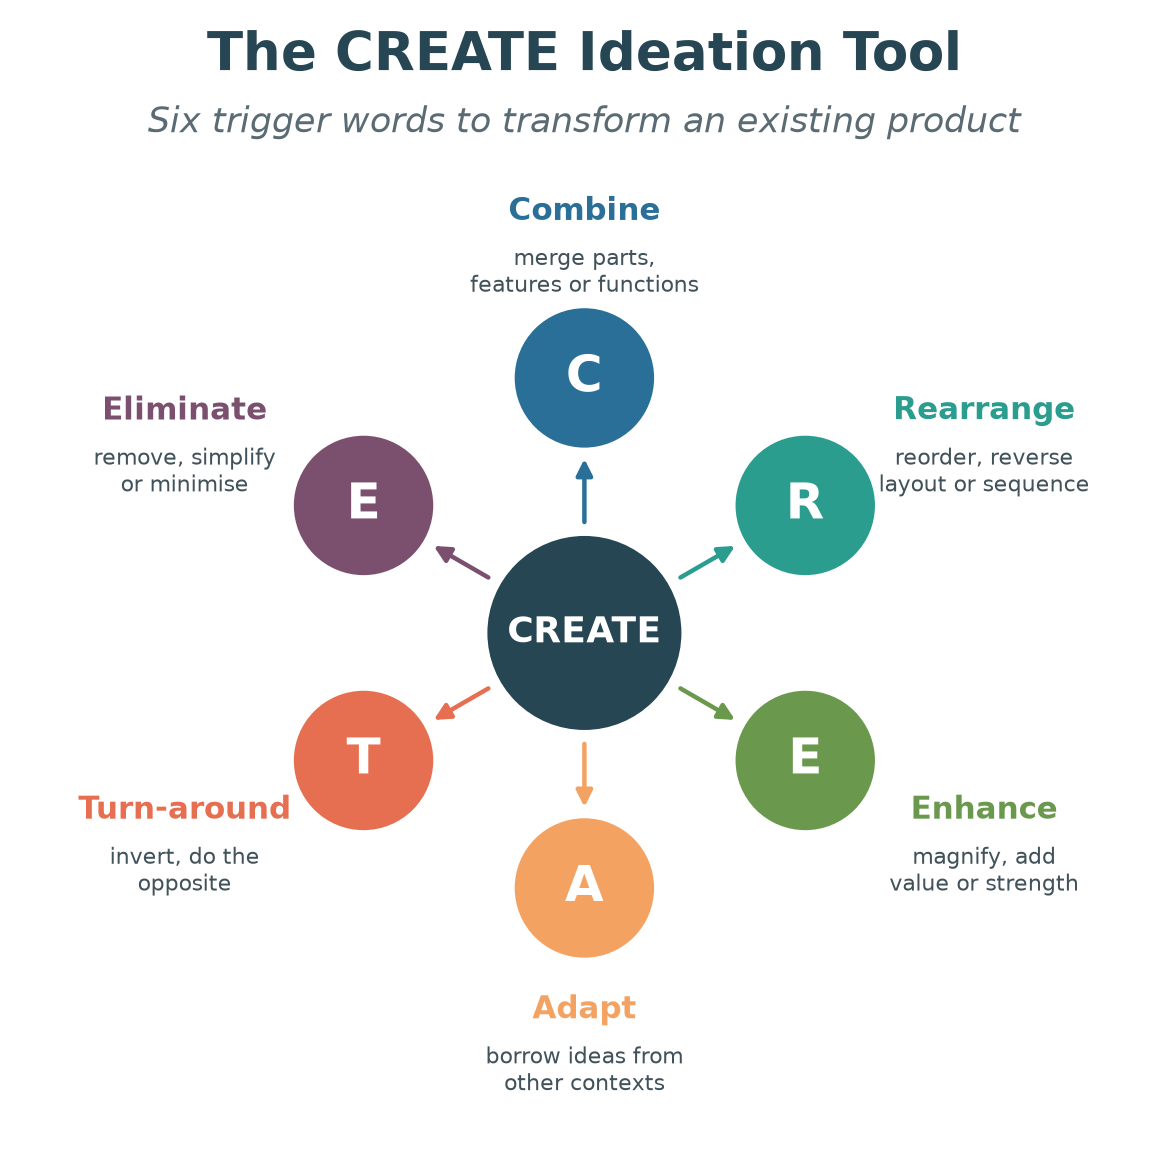
\includegraphics[width=\linewidth]{figures/create_tool.png}
    \end{column}
    \begin{column}{0.45\textwidth}\scriptsize
      \kw{CREATE} is a set of \emph{trigger words} to transform an existing
      product:
      \begin{itemize}\scriptsize
        \item \textbf{C}ombine \quad \textbf{R}earrange
        \item \textbf{E}nhance \quad \textbf{A}dapt
        \item \textbf{T}urn-around \quad \textbf{E}liminate
      \end{itemize}
      \vspace{0.3em}
      Apply each trigger to your problem, then \kwt{draw the product / system}
      that results.
    \end{column}
  \end{columns}
\end{frame}

\begin{frame}{Customer Journey Map (CJM)}
  \bigfig{cjm.png}{Map actions, touch-points, emotions \& pain points — before, during \& after.}
\end{frame}

\begin{frame}{How Might We (HMW) Questions}
  \begin{columns}[c]
    \begin{column}{0.55\textwidth}
      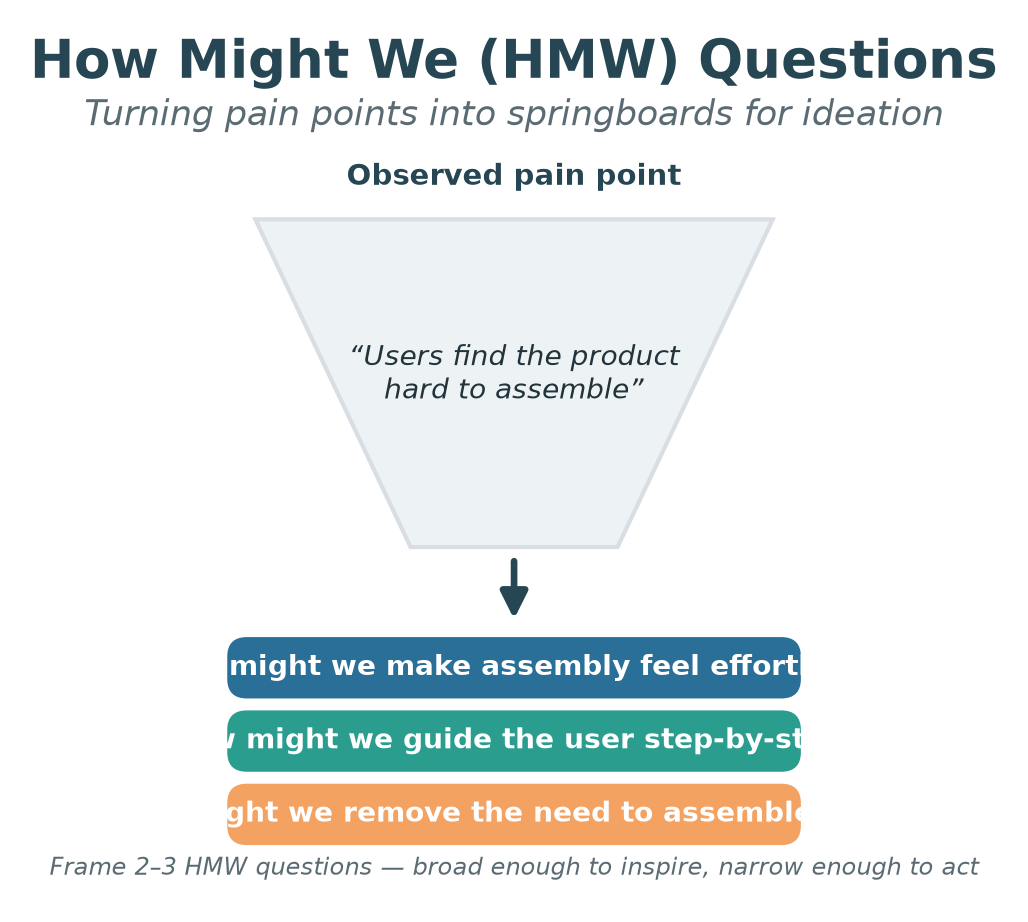
\includegraphics[width=\linewidth]{figures/hmw.png}
    \end{column}
    \begin{column}{0.45\textwidth}\scriptsize
      Turn each \kwc{pain point} from the CJM into an optimistic
      \kw{"How Might We\ldots"} question.
      \vspace{0.3em}
      \begin{itemize}\scriptsize
        \item Broad enough to \emph{inspire} ideas.
        \item Narrow enough to \emph{act} on.
        \item Frame \textbf{2--3} for your mock scenario.
      \end{itemize}
    \end{column}
  \end{columns}
\end{frame}

\begin{frame}{Service Blueprint}
  \bigfig{service_blueprint.png}{Layer the journey with front-stage, back-stage \& support processes; identify touch-points.}
\end{frame}

%==============================================================================
\section*{Wrap-up}
%==============================================================================
\begin{frame}{Bringing It All Together}
  \accentrule\\[0.4em]
  \small
  \begin{columns}[T]
    \begin{column}{0.5\textwidth}
      \begin{itemize}\small
        \item \pill{dtblue}{Unit I} — learn, remember, empathise.
        \item \pill{dtteal}{Unit II} — the design-thinking process.
        \item \pill{dtorange}{Unit III} — design \& prototype products.
      \end{itemize}
    \end{column}
    \begin{column}{0.5\textwidth}
      \begin{itemize}\small
        \item \pill{dtcoral}{Unit IV} — centre on the customer.
        \item \pill{dtplum}{Unit V} — build \& blueprint in the lab.
      \end{itemize}
    \end{column}
  \end{columns}
  \vspace{0.5em}
  \begin{block}{The golden thread}\footnotesize
    Every unit returns to one idea: \textbf{empathise with people, then
    iterate} — observe, frame, ideate, prototype, test, and repeat until the
    experience truly serves the user.
  \end{block}
\end{frame}

\begin{frame}[plain]
  \begin{tikzpicture}[remember picture,overlay]
    \fill[dtnavy] (current page.south west) rectangle (current page.north east);
    \node[text=white,font=\Huge\bfseries] at ([yshift=0.6cm]current page.center) {Thank You};
    \node[text=dtyellow,font=\large] at ([yshift=-0.8cm]current page.center)
      {Design Thinking \& Fabrication Laboratory};
    \node[text=dtsky,font=\footnotesize] at ([yshift=-1.8cm]current page.center)
      {Empathise \textcolor{white}{$\to$} Define \textcolor{white}{$\to$} Ideate \textcolor{white}{$\to$} Prototype \textcolor{white}{$\to$} Test};
  \end{tikzpicture}
\end{frame}

\end{document}
